\chapter{Observations Summary}
\label{chap:observations}

\section{Introduction}

Members of the DTC 1 section observed patients with left neglect at Alexian
Brothers Hospital in Elk Grove Village on Wednesday, January 18, 2023. They
also spoke with Dr. Kate Enzler to get further information about this
condition. The purpose of this observation was to understand the symptoms and
difficulties caused by left neglect, and how the severity can vary. The
observation lasted about an hour. This appendix explains the methodology used
to conduct the observation and what was learned about the condition of left
neglect.

\section{Methodology}

The observation took place in a therapy room, where users typically receive
physical therapy while recovering from a stroke or other brain injuries. The
users were interviewed to get information about their experiences with left
neglect and associated challenges. They were asked what therapies currently
work best for them and which ones don’t. The users were also asked for any
requirements they would have for the device. Then, Dr. Enzler demonstrated some
of the therapy methods she is currently using to treat left neglect.

\section{Results}

\subsection{Cheryl}

The first user is a female who had a stroke on December 19, 2022, which caused
her left neglect and a loss of her left peripheral vision. Her main challenges
are hygiene, reading, and therapy exercises.

\subsubsection{Therapies used}

Cheryl described the following therapies that she had tried. Her therapy was
structured around her love of reading, which helped motivate her.

\begin{description}
\item[Brightly colored lines on the left side of a book] Reminds users to scan
  to the left side of the page.
\item[Lighthouse Technique] Has users look from one shoulder to the other and
  back to scan their entire visual field.
\item[Edge Technique] Gets users to scan the full size of an object by looking
  for its edges.
\item[Finger Tracing Strategy] Has users scan the full shape of an object by
  following its edges.
\item[Guideline Markers] Marks areas to look at/focus on.
\item[Large Print Books] Just helps in general to make reading easier. These
  were partially used because of eyesight concerns.
\end{description}

\subsubsection{Feelings about her care}

Things that helped Cheryl throughout her care were the abundance of options to
choose from (i.e.., books, etc.) and here commitment to reading. The main
difficulties for here were reoccurring feelings of stupidity, as
previously easy tasks were now difficult, and annoyance from her visual field
cut, which felt like a wall to her.

\subsubsection{Observational notes}

The following are some observations noticed while watching Cheryl perform
therapy tasks with Dr. Enzler.
\begin{itemize}
\item Her left peripheral vision is completely gone.
\item She preferred verbal reminders, especially verbal affirmations.
\item Scanning was done both horizontally and vertically.
\end{itemize}

\subsubsection{Product Requirements}

Cheryl listed the following requirements for a product that she would use:
\begin{itemize}
\item High stress situations should be avoided at all costs. Otherwise, she
  wants to simply shut down.
\item Screens (i.e., phones) can be difficult to use. The small text is already
  difficult to read for an elderly person. Additionally, processing the
  information-dense display causes difficulties.
\end{itemize}

\subsection{Bryan}

The second user is a male who had a stroke on December 24, 2022. This caused
left neglect, but no change in vision. He is still in the early stages of
recovery, and is still unsure of his main challenges. He also has baseline ADD
(Attention Deficit Disorder) that has impacted him throughout his life.

\subsubsection{Therapies used}

Bryan, who was earlier in his recovery, had only tried a fraction of the
techniques that Cheryl had used. The ones he did use are documented below.

\begin{description}
\item[Lighthouse technique] Please see above for a description.

\item[Self-reminders] Bryan found it helpful to talk to himself and give
  himself reminders on what to do (i.e., ``look left now'', etc.).
\end{description}

\subsubsection{Observational Notes}

The following are some observations noticed while watching Bryan perform
therapy tasks with Dr. Enzler.

\begin{itemize}
\item He has a subconscious knowledge of Dr. Enzler’s location, gesturing
  directly towards her based on audio cues.
\item An initial scan to left ends about 10 degrees left of center, but with
  repeated reminders he will turn his head over his shoulder.
\item With cross-out puzzles (an exercise where you cross out all objects of
  one shape on the page), he was able to identify most items on a sparse page,
  but more dense pages led to more missed items.
\item Physical stimuli on the left side had little effect.
\item Works very methodically through therapy exercises.
\item Eyes stray right, even when looking left. 
\end{itemize}

\subsubsection{Product Requirements}

Bryan listed the following requirements for a product he would consider using:
\begin{itemize}
\item Keep it simple.
\item Don’t overstimulate.
\item Don’t overstimulate.
\item Don’t make people feel stupid.
\item Make it cheap.
\item Have fun.
\end{itemize}

\section{Conclusion}
The challenges for each user are different, however, they all revolve around a
lack of awareness left of center. Both users responded positively to affirming
expressions, such as “You can do it!”, which may be good to implement in our
product. They also both used the lighthouse technique and found it effective,
meaning it may be a good starting point for our design. Both users also wanted
a simple solution that wouldn’t be overstimulating, meaning it would be useful
if our product was adjustable in terms of amount of stimulus.  The users also
want the device to be easy to use in order to preserve dignity, meaning it
would be good if the device was discrete. Finally, it seems like it would be
very helpful to make the device customizable to the user, as it was said that
the most effective therapies were centered around doing things the user loved.

\begin{figure}[h]
  \centering
  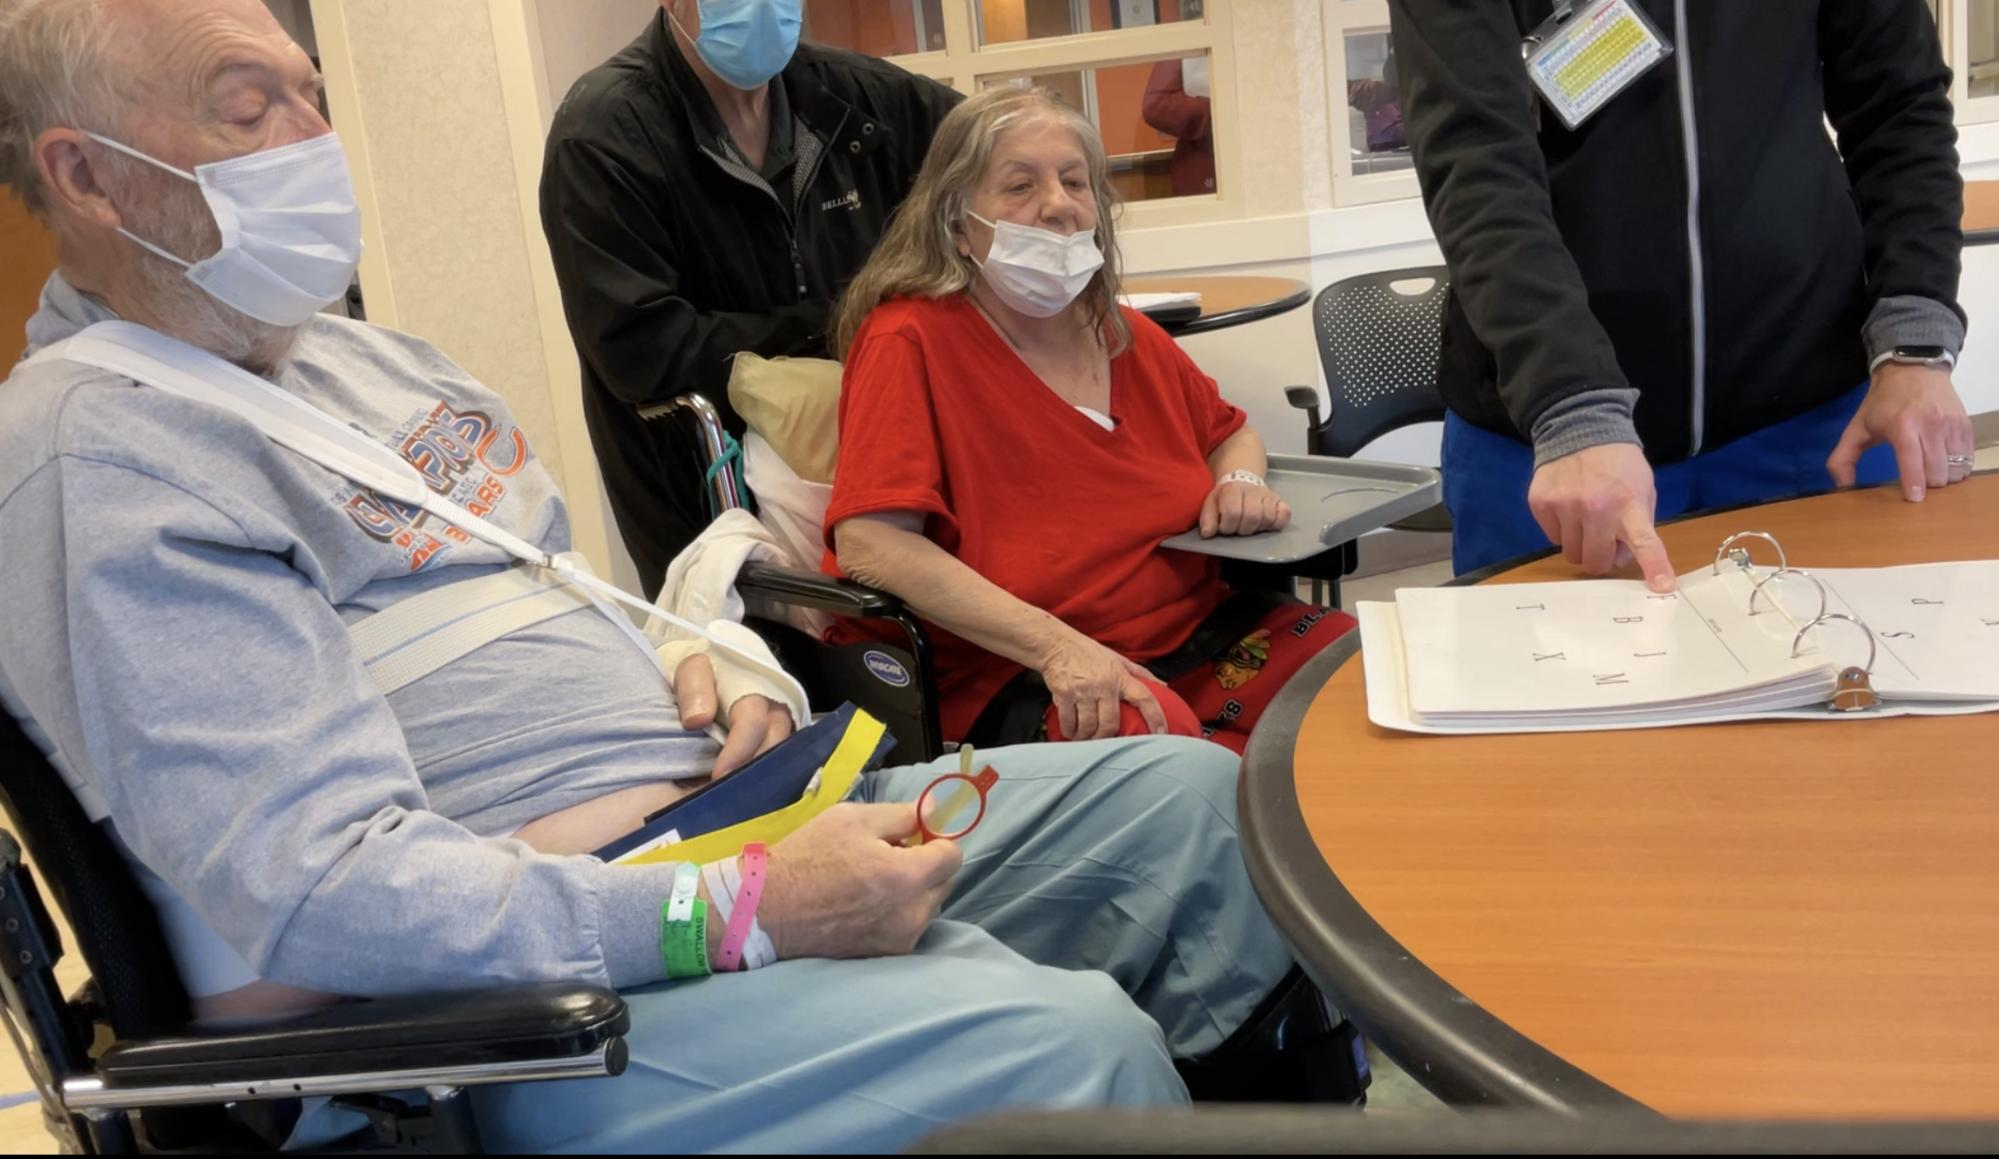
\includegraphics[width=\textwidth]{users}
  \caption{Bryan and Cheryl, the two patients we observed and interviewed.}
\end{figure}

%%% Local Variables:
%%% mode: latex
%%% TeX-master: "../final_report"
%%% End:
